\graphicspath{{figures/appendix/}}

\begin{mclistof}{List of Abbreviations}{3.2cm}

\item[aaRS] Aminoacyl-tRNA synthetase

\item[ABC] ATP-binding cassette

\item[ADP] Adenosine diphosphate

\item[ATP] Adenosine triphosphate

\item[ANAP] L-3-(6-acetylnaphthalen-2-ylamino)-2-aminopropionic acid

\item[BK channel] Large conductance K\textsuperscript{+} channel

\item[CFTR] Cystic fibrosis transmembrane conductance regulator

\item[CNG channel] Cyclic nucleotide gated channel

\item[Cryo-EM] Cryo-electron microscopy

\item[DEND syndrome] Permanent neonatal diabetes mellitus with neurological complications

\item[EC\textsubscript{50}] Half maximal effective concentration

\item[ELPD] Expected log pointwise predictive density

\item[ER] Endoplasmic reticulum

\item[FRET] F\"{o}rster resonance energy transfer

\item[GFP] Green fluorescent protein

\item[HA] Human influenza hemagglutinin

\item[HEK293T] Human embryonic kidney 293 cells containing the SV40 T-antigen

\item[HRP] Horseradish peroxidase

\item[IC\textsubscript{50}] Half maximal inhibitory concentration

\item[K\ATP{} channel] ATP-sensitive potassium channel

\item[Kir] Inward rectifier potassium channel

\item[L0] Loop zero

\item[LOO-CV] Leave-one-out cross-validation

\item[mO] mOrange fluorescent protein

\item[MWC] Monod-Wyman-Changeaux

\item[nAChR] Nicotinic acetylcholine receptor

\item[NBD] Nucleotide binding domain

\item[PCF] Patch-clamp fluorometry

\item[PDB] Protein data bank

\item[PIP\textsubscript{2}] Phosphatidylinositol 4,5-bisphosphate

\item[$P_O$] Open probability

\item[PPIs] Phosphoinositides

\item[SUR] Sulphonylurea receptor

\item[TEA\textsuperscript{+}] Triethylammonium ion

\item[TMD] Transmembrane domain

\item[TNP-ADP] Trinitrophenyl adenosine diphosphate

\item[TNP-ATP] Trinitrophenyl adenosine triphosphate

\item[tRNA] Transfer RNA

\item[UAA] Unnatural amino acid

\item[WT] Wild-type

\end{mclistof}

\begin{figure}[h]
	\centering
	\begin{subfigure}[t]{0.45\textwidth}
		\caption{}\label{ch0fig:kir_constructs}
		\centering
		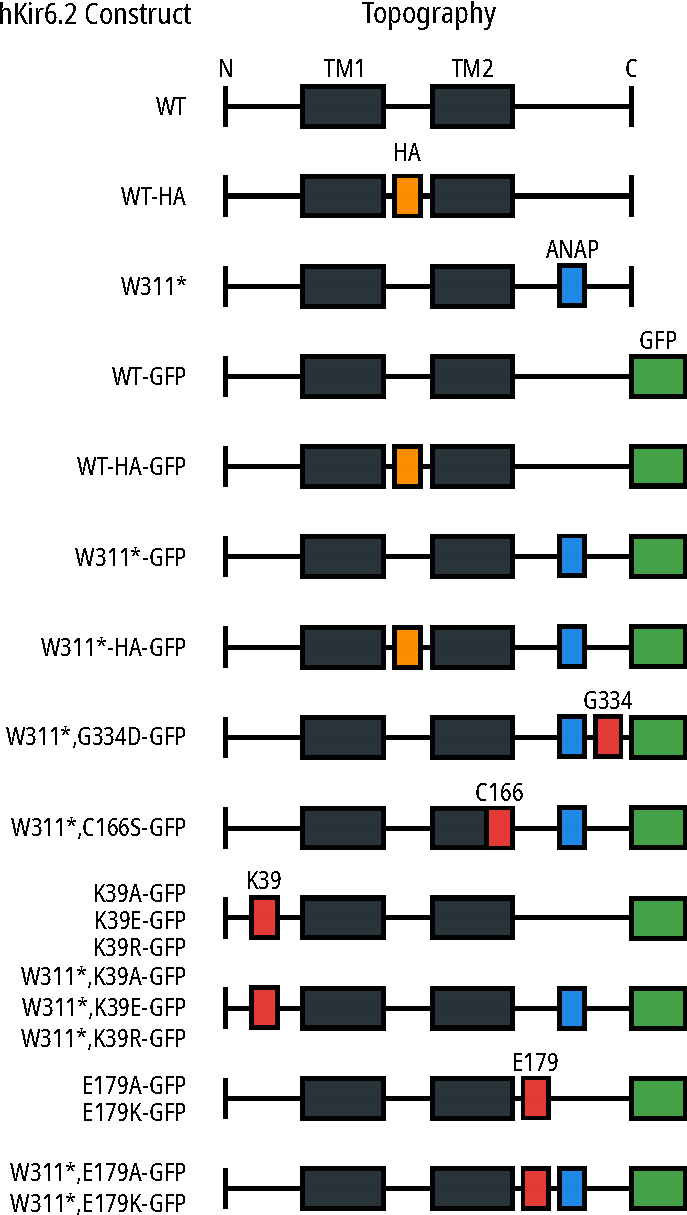
\includegraphics[width=\textwidth]{kir_constructs.pdf}
	\end{subfigure}
	\hfill
	\begin{subfigure}[t]{0.45\textwidth}
		\caption{}\label{ch0fig:sur_constructs}
		\centering
		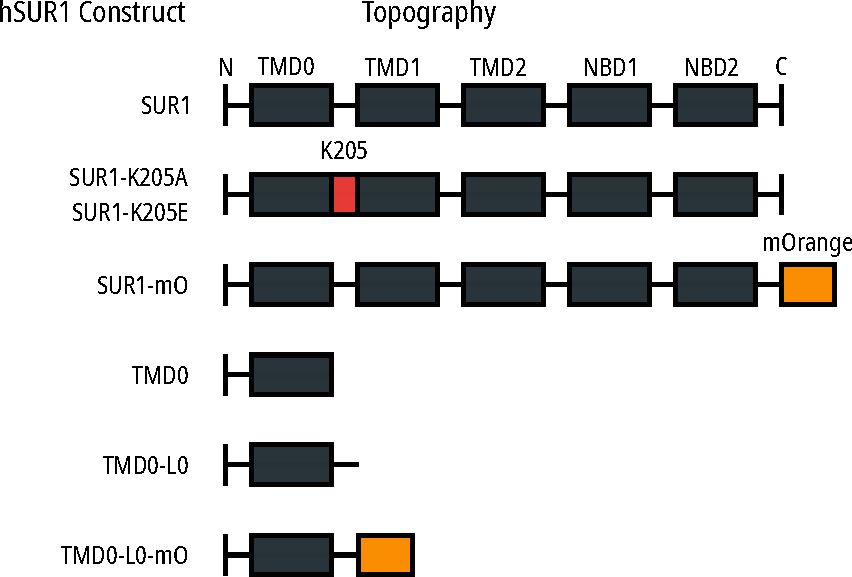
\includegraphics[width=\textwidth]{sur_constructs.pdf}
	\end{subfigure}
	\caption[hKir6.2 and hSUR1 constructs and their abbreviations]{
	{\bf\mccorrect{hKir6.2 and hSUR1 constructs and their abbreviations.}}
	Topographical diagrams of the constructs used in this thesis.
	Transmembrane domains (TMDs) are indicated with dark grey rectangles, and the various insertions and substitutions are shown as labelled coloured rectangles.
	Kir6.2 constructs are shown in panel \subref{ch0fig:kir_constructs}, SUR1 constructs in panel \subref{ch0fig:sur_constructs}.
	}\label{ch0fig:constructs}
\end{figure}